\documentclass[11pt,oneside,letterpaper]{article}

% graphicx package, useful for including eps and pdf graphics
\usepackage{graphicx}
\DeclareGraphicsExtensions{.pdf,.png,.jpg}

% basic packages
\usepackage{color} 
\usepackage{parskip}
\usepackage{float}

% text layout
\usepackage{geometry}
\geometry{textwidth=15cm} % 15.25cm for single-space, 16.25cm for double-space
\geometry{textheight=22cm} % 22cm for single-space, 22.5cm for double-space

% helps to keep figures from being orphaned on a page by themselves
\renewcommand{\topfraction}{0.85}
\renewcommand{\textfraction}{0.1}

% bold the 'Figure #' in the caption and separate it with a period
% Captions will be left justified
\usepackage[labelfont=bf,labelsep=period,font=small]{caption}

% review layout with double-spacing
%\usepackage{setspace} 
%\doublespacing
%\captionsetup{labelfont=bf,labelsep=period,font=doublespacing}

% cite package, to clean up citations in the main text. Do not remove.
\usepackage{cite}
%\renewcommand\citeleft{(}
%\renewcommand\citeright{)}
%\renewcommand\citeform[1]{\textsl{#1}}

% Remove brackets from numbering in list of References
\renewcommand\refname{\large References}
\makeatletter
\renewcommand{\@biblabel}[1]{\quad#1.}
\makeatother

%\usepackage{authblk}
%\renewcommand\Authands{ \& }
%\renewcommand\Authfont{\normalsize \bf}
%\renewcommand\Affilfont{\small \normalfont}

% math notation
\usepackage{amssymb}
\newcommand{\point}{f_{\scriptscriptstyle \vert}}
\newcommand{\threshold}{f_{\textstyle \lrcorner}}
\newcommand{\interval}{f_{\sqcup}}

% comments
\usepackage{ulem}
\definecolor{purple}{rgb}{0.459,0.109,0.538}
\def\tb#1#2{\sout{#1} \textcolor{purple}{#2}} 
\def\tbc#1{\textcolor{purple}{[#1]}}

%%% TITLE %%%
\title{\vspace{1.0cm} \LARGE \bf Integrating influenza antigenic dynamics with molecular evolution}
\author{}
\date{}

\begin{document}

\maketitle

%%% ABSTRACT %%%
\section*{Abstract}

%%% INTRODUCTION %%%
\section*{Introduction}

Seasonal influenza infects between 10\% and 20\% of the human population every year, causing 250,000 to 500,000 deaths annually \cite{flufactsheet}. 
While individuals develop long-lasting immunity to particular influenza strains after infection, antigenic mutations to the influenza virus genome result in proteins that are recognized to a lesser degree by the human immune system, leaving individuals susceptible to future infection. 
The influenza virus population continually evolves in antigenic phenotype in a process known as antigenic drift. 
A large proportion of the disease burden of influenza stems from antigenic drift; it is why vaccines remain only transiently effective. 
A thorough understanding of the process of antigenic drift is essential to our efforts to control mortality and morbidity through the use of a seasonal influenza vaccine.

There are currently three major clades of influenza circulating within the human population: influenza A subtype H3N2, influenza A subtype H1N1 and influenza B. 
Subtypes refer to the genes, hemagglutinin (H or HA) and neuraminidase (N or NA), that are primarily responsible for the antigenic character of a strain. 
Currently, seasonal influenza is treated with a trivalent vaccine containing one strain of H3N2, one strain of H1N1 and one strain of influenza B. 
The World Health Organization (WHO) Global Influenza Surveillance Network issues twice-yearly recommendations on which strains of influenza to use as vaccine strains in 9--12 month’s time, i.e.\ a February recommendation for the Northern Hemisphere flu season and an August recommendation for the Southern Hemisphere flu season. 
These recommendations are provided by a panel of experts after review of the available data.

Mutations to the HA1 region of the hemagglutinin protein are thought to drive the majority of antigenic drift in the influenza virus \cite{Nelson07NatRevGenet}. 
Experimental characterization of antigenic phenotype is possible through the hemagglutination inhibition (HI) assay \cite{Hirst43}, which measures the cross-reactivity of one virus strain to serum raised against another strain. 
Sera from older strains react poorly with more evolved viruses resulting in new strains having a transmission advantage over established strains. 
The results of many HI assays across a multitude of virus strains can be combined to yield a two-dimensional map, quantifying antigenic similarity and distance \cite{Smith04}. 
The antigenic map of influenza A (H3N2) has shown largely linear movement of the influenza virus population since its introduction in 1968. 
Evolution of antigenic phenotype appears punctuated with periods of stasis interspersed by periods of more rapid innovation, while genetic evolution appears more continuous \cite{Smith04}, suggesting that a relatively small number of genetic changes or combinations of genetic changes may drive changes in antigenic phenotype. 
The process of antigenic drift results in the rapid turnover of the virus population. 
Although mutation occurs rapidly, standing genetic diversity is low and phylogenetic analysis shows a characteristically `spindly' tree with a single predominant trunk lineage and transitory side branches that persist for only 1--5 years \cite{Fitch97}.

Previously, the antigenic and genetic patterns of influenza evolution have been analyzed essentially in isolation. 
An antigenic map is constructed from a panel of HI measurements, and a phylogenetic tree is constructed from sequence data. 
However, the opportunity for a combined approach exists as both the antigenic map and the phylogenetic tree often contain many of the same isolates. 
Here, we implement a flexible Bayesian approach to jointly analyze the antigenic and genetic dynamics of the influenza virus population. 
We apply this approach to investigate the dynamics of influenza lineages A/H3N2,  A/H1N1, B/Victoria and B/Yamagata. 

%%% RESULTS %%%
\section*{Results}

\subsection*{Bayesian multidimensional scaling}

In order to assess patterns of antigenic evolution among influenza strains, we implemented a Bayesian probabilistic analog of multidimensional scaling, referred to here as BMDS.
In this model, viruses and sera are given $N$ dimensional locations, thus specifying an `antigenic map', such that distances between viruses and sera in this space are inversely proportional to cross-reactivity.
In the BMDS model, a map distance of one antigenic unit translates to an expectation of a 2-fold drop in HI titer between virus and sera.
Maps that produce pairwise distances most congruent with the observed titers will have a high likelihood and will be favored by the BMDS model.
We integrate over sources of uncertainty, such as antigenic locations, in a flexible Bayesian fashion.

We began with a BMDS analog of the MDS model used by Smith et al. \cite{Smith04}, where viruses and sera are represented as 2D locations and HI expectation is relative to the maximum titer of a particular ferret sera.
This model performed well, yielding an average absolute predictive error of 0.66 log$_2$ HI titers on the 6545 training measurements used to build the model, and an average error of 0.86 on an additional 723 test measurements (Table \ref{errortable}).
We find that a model with two dimensional antigenic locations better predicts test data than models with higher (or lower) dimensionality (Table \ref{errortable}), and thus specify a two dimensional model in all subsequent analyses.
We extend this model by estimating the strength of overall reactivity of each sera rather than fixing this at the maximum titer, and additionally, by estimating the strength of reactivity of each virus in calculating an expectated HI titer.
We refer to these estimates as column effects and row effects, respectively.
We found that including these effects decreased training error to 0.50 and test error to 0.75 log$_2$ HI titers.

%%% errortable %%%
\begin{table}[tb]
	\centering
	\caption{\textbf{Absolute prediction error of log$_2$ HI titer for training and test data across models.}}
	\label{errortable}
	\begin{tabular}{ c c c c c } 
	\hline
	MDS 	& 	Column effects 	&	Row effects	& 	Training error	& 	Test error	\\
	\hline	
	1D 		&	Fixed 			&	None		& 	0.91			&	1.03		\\	
	2D 		&	Fixed 			&	None		& 	0.66			&	0.86		\\
	3D 		&	Fixed 			&	None		& 	0.65			&	0.88		\\
	4D 		&	Fixed 			&	None		& 	0.71			&	0.96		\\
	5D 		&	Fixed 			&	None		& 	0.71			&	1.06		\\	
	2D 		&	Estimated 		&	None		& 	0.55			&	0.77		\\	
	2D 		&	Estimated 		&	Estimated	& 	0.50			&	0.75		\\		
	\hline
	\end{tabular}
\end{table}

\subsection*{Antigenic drift across influenza lineages}

% Antigenic drift with 95% CI
% H3N2: 1.159 (1.126-1.203)
% H1N1: 0.643 (0.585-0.703)
% Vic:  0.449 (0.397-0.506)
% Yam:  0.203 (0.150-0.260)

Through this analysis we find that the antigenic phenotype of influenza A (H3N2) underwent rapid turnover from 1968 to 2011 (Figure~\ref{flu_grid}A).  
Here, cross-reactive measurements only exist betwen strains sampled at most 11 years apart, leaving only threshold titers, e.g.\ `$<$40', in more temporally distant comparisons.  
Because of the threshold of sensitivity of the HI assay, it's impossible to distinguish a linear trajectory in 2D antigenic space, from a curved trajectory, so long as the curve does not bring antigenic phenotype full circle to have cross-reactive measurements between temporally distant strains.
To solve this problem of identifiability, we assumed a weak prior that favors linear movement in the 2D antigenic space, with the slope of the linear relationship and the precision of the relationship incorporated into the Bayesian model (see Methods).

We find that influenza A (H3N2) evolved 1.16 antigenic units per year from 1968 to 2011, with 95\% highest posterior density (HPD) interval 1.13--1.20 (Figure~\ref{flu_grid}C).
However, the rate of antigenic drift was not constant, with year-to-year movement of mean antigenic phenotype showing an interquartile range of 0.40--1.79.  
Large jumps in antigenic phenotype (Figure~\ref{flu_grid}C) correspond to cluster transitions identified by Smith et al. \cite{Smith04}.  
Most variation is contained within the first antigenic dimension, but dimension 2 ocassionally shows variation when two antigenically distinct lineages emerge and transiently coexist (Figure~\ref{flu_grid}E), as is the case with the previously identified Beijing 1989 and Beijing 1992 clusters.

We find that other types and subtypes of influenza evolved in antigenic phenotype substantially slower than influenza A (H3N2).
Influenza A (H1N1) evolved at an average rate of 0.64 antigenic units per year (HPD 0.59--0.70) since its reemergence in 1977 to 2009.  
H1N1 influenza shows a similar pattern of punctuated antigenic evolution with occasional larger jumps in phenotype, such as the emergence of the Solomon Islands 2006 cluster.  
It is unclear whether H1N1 undergoes fewer antigenic transitions of comparable magnitude to H3N2, or whether antigenic transitions in H1N1 are of smaller scale.  
Both the Victoria and Yamagata lineages of influenza B also evolved relatively slowely, with average rates of 0.45 (HPD 0.40--0.51) and 0.20 (HPD 0.15--0.26) antigenic units per year, respectively.  
From 2000 to 2011, both the Victoria and Yamagata lineages show slow antigenic movement, but no major antigenic transitions.

%%% flu_grid %%%
\begin{figure}[tb]
	\centering		
	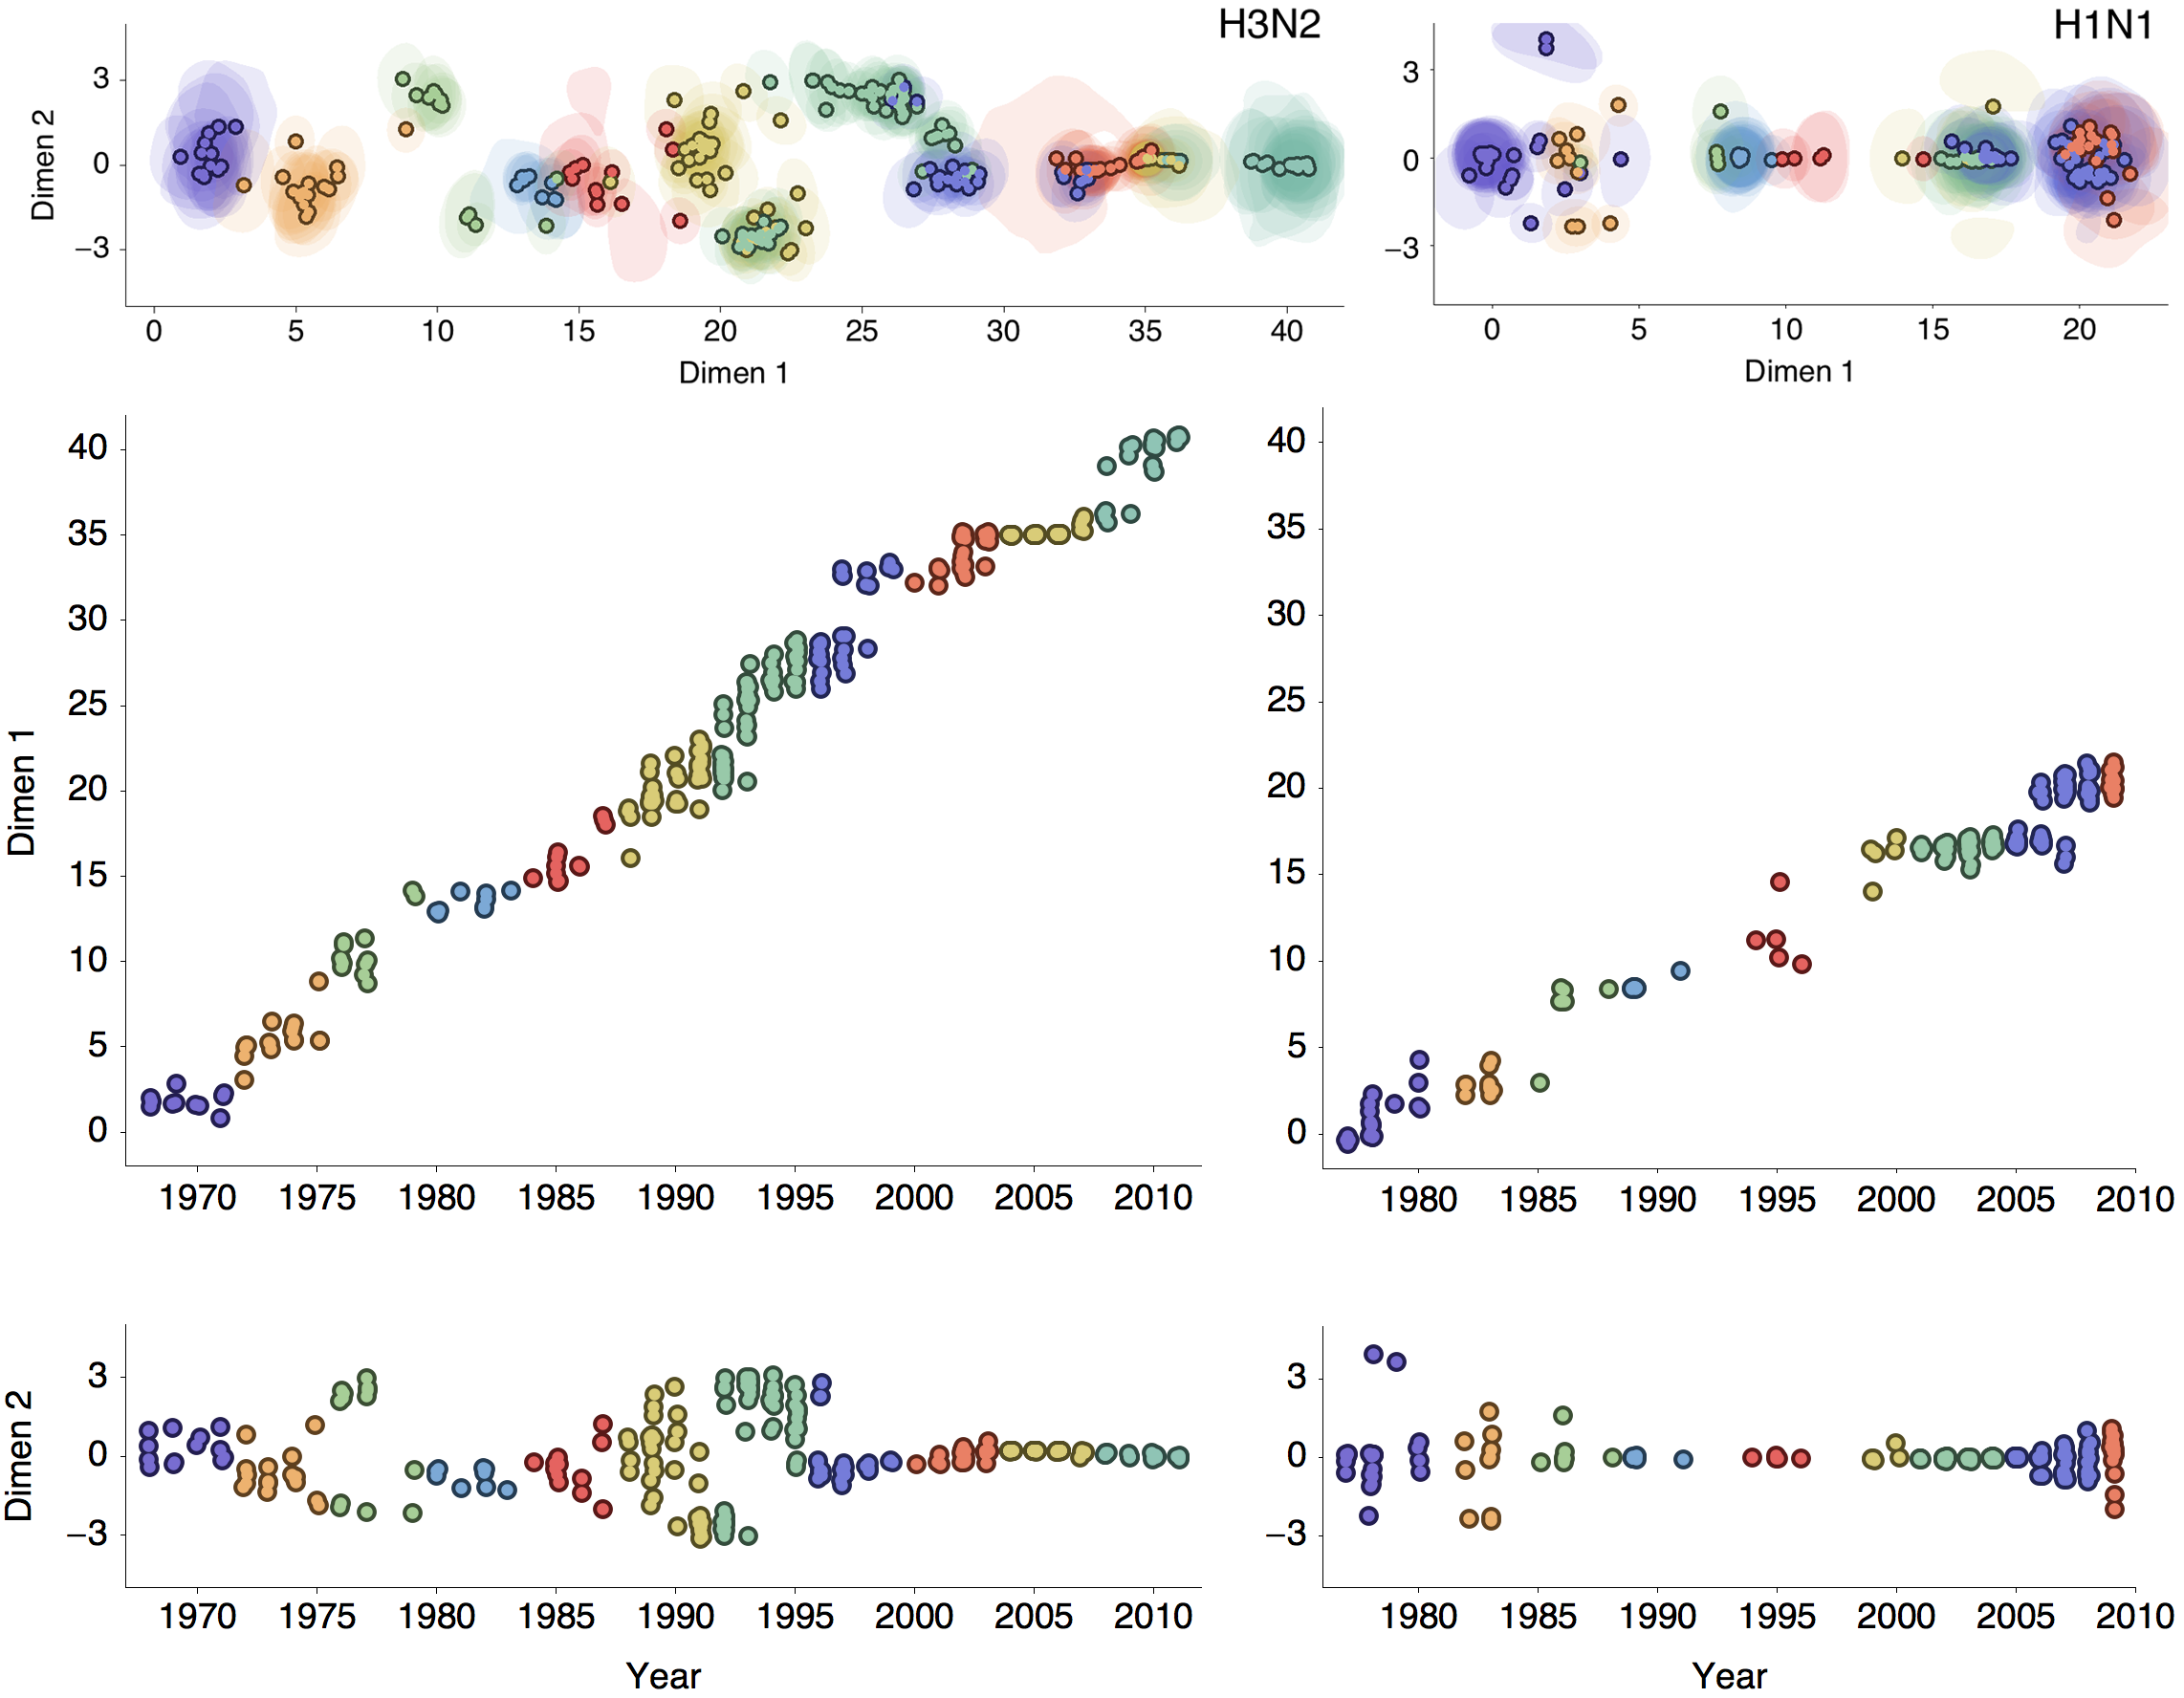
\includegraphics[width=\textwidth]{figures/flu_grid}
	\caption{\textbf{Antigenic locations of influenza H3N2 and H1N1.} 
	(A) and (B) Antigenic maps showing the mean posterior location of 338 strains of H3N2 influenza and 243 strains of H1N1 influenza.  
	The model has been constructed so that the primary axis of variation lies along the $x$-axis (AG1), with the $y$-axis (AG2) orthogonal to this axis.  
	(C) and (D) Antigenic location along the primary axis of variation (AG1) vs.\ year of virus isolation.  
	The dashed lines show the relationship of between time and AG1 with a slope of \tbc{XXX} for H3N2 and \tbc{XXX} for H1N1.  
	(E) and (F) Antigenic location along the secondary axis of variation (AG2) vs.\ year of virus isolation.  
	Points represent median strain locations and translucent areas represent 50\% highest density regions.
	Antigenic units represent two-fold dilutions of the HI assay, and strains have been colored based on year of isolation.} 
	\label{flu_grid} 
\end{figure}

\subsection*{Competition between influenza lineages}

We investigated the relative rates of antigenic evolution in different influenza lineages from 1999 to 2009, finding a general correspondence between antigenic drift along antigenic dimension 1 and relative incidence between influenza A/H3N2, A/H1N1, B/Victoria and B/Yamagata.
From 1999 to 2009, influenza A (H3N2) accounted for the majority of antigenic evolution (51\%), while A/H1N1, B/Victoria and B/Yamagata split the remainder, accounting for 17\%, 18\% and 14\%, respectively.
Similarly, influenza A (H3N2) was responsible for the majority of incidence (54\%) in the USA during this time period.
Influenza A (H1N1) accounted for 23\% of incidence, B/Victoria accounted for 12\% of incidence and B/Yamagata accounted for 10\% of incidence.
These proportions are significantly similar to one another (randomization test $p = 0.010$).


%%% drift_incidence %%%
\begin{figure}[tb]
	\centering		
	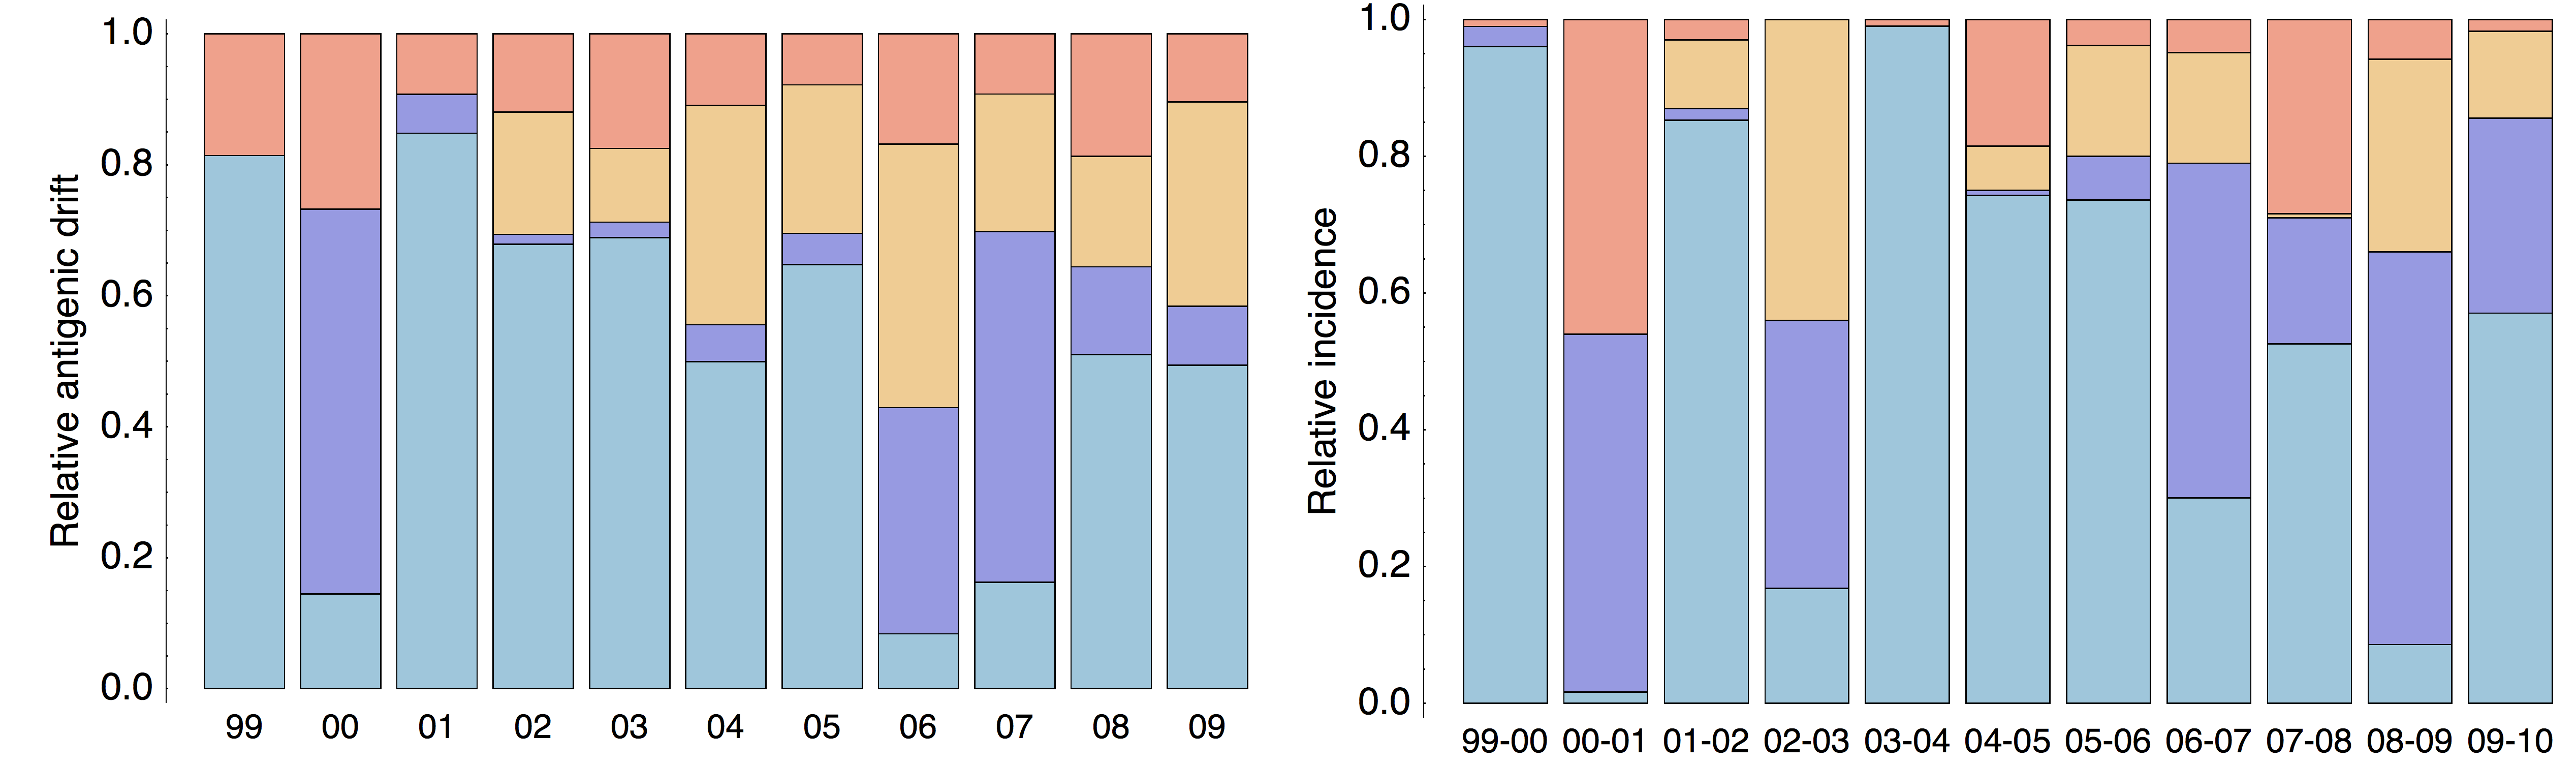
\includegraphics[width=\textwidth]{figures/drift_incidence}
	\caption{\textbf{Relative antigenic drift and incidence between lineages of influenza from 1999 to 2009.} 
	(A) Relative antigenic drift of influenza A H3N2 and H1N1 and influenza B Victoria and Yamagata lineages.
	Relative change in antigenic dimension 1 between year $i$ and year $i-1$ is shown for each of the 4 lineages.
	(B) Relative incidence of influenza A H3N2 and H1N1 and influenza B Victoria and Yamagata lineages.
	Relative isolation counts of each lineage in the USA for each winter influenza season.
	} 
	\label{drift_incidence} 
\end{figure}

%%% DISCUSSION %%%
\section*{Discussion}

%%% METHODS %%%
\section*{Methods}

\subsection*{Genetic and antigenic data}

We compiled an antigenic dataset for hemagglutination inhibition (HI) measurements for influenza A (H3N2) by combining data used in Hay et al. \cite{Hay01}, Smith et al.\ \cite{Smith04}, Russell et al.\ \cite{Russell08}, Barr et al.\ \cite{Barr10} and Cox et al.\ \tbc{WHO report}. 
This combined dataset had 1651 influenza isolates (present as either virus or sera in HI comparisons) dating from 1968 to 2011. 
However, the majority of isolates date from 2002 to 2007. 
Because we are interested in longer-term antigenic evolution, we censored the data to have at most 20 strains per year, preferentially keeping those strains with more antigenic comparisons. 
This censoring left 338 strains present as 320 viruses and 438 sera (replicate sera are often constructed from the same strain). 
Across these viruses and sera, we observe 7240 HI measurements. 
We queried the IRD \cite{IRD} and GISAID \tbc{CITE} sequence databases for HA nucleotide sequences based on strain names, e.g.\ A/HongKong/1/1968, of these strains. 
If a strain had multiple sequences in the databases we preferentially kept the IRD sequence and preferentially kept the longest sequence in IRD. 
Sequences were aligned using MUSCLE v3.7 under default parameters \cite{MUSCLE}.

Antigenic data for influenza A (H1N1) was collected from \cite{Faress05,Chakraverty82,Chakraverty86,Cox83,Daniels85,Daum02,Donatelli93,Kendal78,McDonald07,Nakajima79,Nakajima81,Pereira82,Stevens87,Webster79,Raymond86}.

\subsection*{Bayesian multidimensional scaling}

We follow Smith et al. \cite{Smith04} and represent antigenic locations on a 2D antigenic map. 
Through the hemagglutination inhibition (HI) assay, there exist measurements of the cross-reactivity of hemagglutinin (HA) from one virus strain to serum raised against another strain \cite{Hirst43}. 
Thus, antigenic phenotype is measured through a series a pairwise comparisons $H_{ij}$, comparing virus from strain $i$ to serum from strain $j$. 
Due to experimental constraints, the distance matrix $\mathbf{H}$ is sparse; most comparisons have not be made. 
Our goal is to find an optimal projection of the high-dimensional distance matrix into a lower number of dimensions. 
We conduct this projection using Bayesian multidimensional scaling (BMDS) \cite{Oh01} in which a probabilistic model is constructed to quantify the fit of a particular configuration of cartographic locations to the observed matrix of HI measurements.

Let $X_i \in \Re^{P}$ represent the cartographic location of virus $i$ for $i = 1,\ldots, n$, and $Y_j$ represent the cartographic location of serum $j$ for $j = 1,\ldots, s$.
Virus and antiserum may be isolated from / raised against the same strain and have different cartographic locations.
Typically, $P = 2$, but higher or lower dimensions may better reflect the data.  
This gives set of distances between virus and serum cartographic locations 
\begin{equation}
	\delta_{ij} =  || X_i - Y_j ||_2.
\end{equation}
Here, $H_{ij}$ represents the $\mathrm{log}_2$ HI titer of virus $i$ against serum $j$, and HI distance is defined as
\begin{equation}
	d_{ij} =  \max{ H_j } - H_{ij}.
\end{equation}
Traditionally, the goal of multidimensional scaling (MDS) optimizes over $\mathbf{X}$ and $\mathbf{Y}$ such that
\begin{equation}
	\sum_{(i,j) \in \cal I} 
	\left(
		\delta_{ij} - d_{ij}
	\right)^2
\end{equation}
is minimized, where $\cal I = \{ (i,j) : H_{ij} \mbox{ is measured} \}$. 
Here, we instead assume a probabilistic interpretation in which a point estimate of HI distance is normally distributed 
\begin{equation} 
	d_{ij} \sim \mbox{Normal}( \delta_{ij}, \sigma^2 ),
\end{equation}
and the likelihood of observing some HI distance given the placement of antigenic locations is 
\begin{equation} 
	\point(d_{ij}) = \phi \left( \frac{x-\delta_{ij}}{\sigma} \right),
\end{equation}
where $\sigma^2$ represents variance and $\phi(\cdot)$ represents the standard normal PDF.
However, HI assays sometimes show no inhibition of agglutination at all measured titrations, e.g.\ a measurement can be reported as `$<$40'.
In this case, the likelihood of observing the threshold measurement follows the cumulative density of the upper tail of the normal distribution
\begin{equation} 
	\threshold(d_{ij}) = 1 - \Phi \left( \frac{x-\delta_{ij}}{\sigma} \right),
\end{equation}
where $\Phi(\cdot)$ represents the standard normal CDF.
Although it is simplest to assume that HI measurements represent point estimates, it seems more natural to assume that the threshold for inhibition occurs between two titers, e.g.\ we observe inhibition at 1:40 dilution and no inhibition at 1:80.
Rather taking the HI titer as 1:40, we can instead treat this as an interval measurement, assuming that the exact HI titer for this measurement would occur somewhere between 1:40 and 1:80.
Assuming an HI distance represents an interval estimate, we calculcate its probability according to
\begin{equation} 
	\interval(d_{ij}) = \Phi \left( \frac{x-\delta_{ij}}{\sigma} \right) - \Phi \left( \frac{x-\delta_{ij}-1}{\sigma} \right).
\end{equation}
Throughout the analysis, we use interval probabilities $\interval$ rather than point probabilities $\point$ unless otherwise noted.

We calculcate the likelihood of a set of antigenic locations by multiplying probabilities of individual measurements
\begin{equation} 
	L(\mathbf{X}) = \prod_{(i,j) \in \cal I} f(d_{ij}),
\end{equation}
using probability functions $\point$, $\threshold$ and $\interval$ as appropriate.
We assume that the prior precision $\omega = 1/\sigma^2$ follows a diffuse $\mbox{Gamma}(a, b)$ distribution with $a=0.001$ and $b=1000$, and we assume a uniform prior over $\mathbf{X}$ and $\mathbf{Y}$.

The preceding model represents HI distance as a drop in titer against the most reactive comparison for a particular antiserum.  
Here, we relax this assumption and treat the expected homologous titer as a random variable.
In this case, HI distance follows
\begin{equation} 
	d_{ij} =  C_j - H_{ij},
\end{equation}
with the set of column effects $C_j$ for $j = 1,\ldots, s$ estimated.
We assume that $C_j$ values are hierarchically distributed according to a normal distribution.
The mean value of this distribution is taken from the empirical mean across columns in the $\mathrm{log}_2$ HI matrix, and the variance across sera is estimated.
This formulation assumes that particular sera are more reactive in general than other sera, we follow the same logic and by including an effective of a particular viruses being more reactive in general than other viruses.
Here, HI distance follows
\begin{equation} 
	d_{ij} =  \frac{1}{2} (R_i+C_j) - H_{ij},
\end{equation}
and the set of row effects $R_i$ for $i = 1,\ldots, n$ is modeled in an analogous hierarchical fashion, with the variance across viruses estimated.
We assume separate Gamma(0.001,1000) hyperpriors on the precisions of the $C$ and $R$ distributions.

We integrate over uncertainty using the Markov chain Monto Carlo (MCMC) procedures implemented in the phylogenetic package BEAST. Metropolis-Hastings proposals include moves to individual virus and serum locations $X_i$ and $Y_j$, moves to MDS precision $\omega$ and moves to $C$ and $R$ precision.

%%% ACKNOWLEDGMENTS %%%
\subsection*{Acknowledgments} 

%%% FUNDING %%%
\subsection*{Funding} 

%%% REFERENCES %%%
\bibliographystyle{plos}
\bibliography{flux}

\pagebreak

\setcounter{figure}{0}
\setcounter{table}{0}
\setcounter{page}{1}
\renewcommand{\thefigure}{S\arabic{figure}}
\renewcommand{\thetable}{S\arabic{table}}
\renewcommand{\thepage}{S\arabic{page}}

%%% SUPPORTING INFORMATION %%%
\section*{Supporting Information}

\pagebreak

\end{document}
